\chapter{Experiment}
\label{ch:experiment}

Indien een bepaald framework boven een bepaalde scoregrens ligt zal deze worden opgenomen in het experiment.
Voor het experiment zal een simpele applicatie worden ontwikkelt (touch op het scherm creëert een object) voor elk framework a.h.v. deze applicatie zullen dan volgende kenmerken worden gemeten: startuptijd, CPU load, FPS, memory usage, batterijverbruikt (?) en temperatuur (indien mogelijk).

Indien ik informatie vindt over het automatisch testen van AR applicaties zal deze ook hier terecht komen. Ook zal dit een invloed hebben op het uitvoeren van de experimenten. Als ik hierover bruikbare informatie vind zal ik deze ook gebruiken om het experiment meerdere malen uit te voeren i.p.v. het gelimiteerde aantal keren indien ik het manueel moet doen.

\section{Uitleg experiment}
Hierin komt de uitleg over het experiment zelf, waar dit is uitgevoerd (belichting etc) en hoe ze het kunnen nadoen (link naar applicatie code?).

\section{Startup tijd}
Zou normaal geautomatiseerd kunnen worden! A.h.v. bv een Debug.Log te plaatsen
\section{CPU belasting}
Sommatie nemen van de gemiddelde van elk tijdstip van elk experiment.
\begin{figure}
    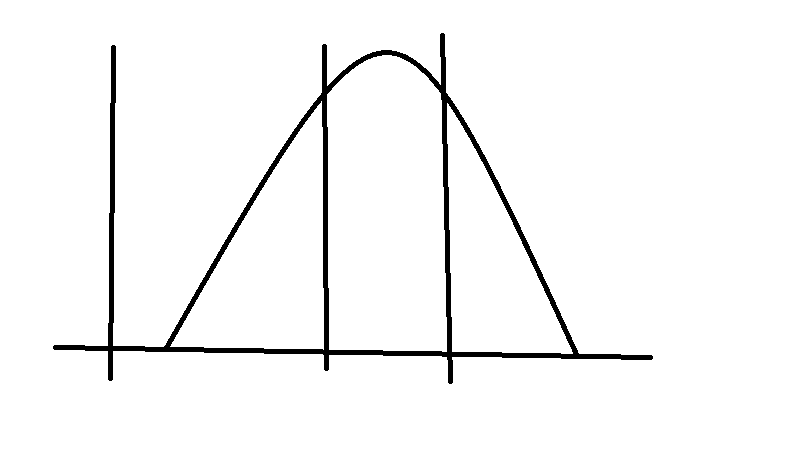
\includegraphics[width=\textwidth]{img/normaleverdeling}\caption{CPU Belasting Van ARCore}\label{fig:cpu1}
\end{figure}
\section{FPS}
Wat belangrijk is bij het meten van FPS is het vermelden van de laagste FPS drop omdat dit eigenlijk het meeste invloed heeft op de ervaring van gebruikers.

Zeggen wat elke drop in FPS betekent indien deze te verklaren is. BV: de drop die men kan zien na 5 min is wanneer er in de applicatie een gameobject werd aangemaakt. OF misschien in het begin van het experiment een tijdstabel zetten wanneer welke actie wordt gedaan?

Uit de data van beide frameworks blijkt het dat Vuforia maximum 60 FPS kan halen terwijl ARCore maar een maximum behaalt van 30 FPS. Het halen van een 60 FPS is redelijk onbelangrijk omdat vele Android Smartphones (vooral de iets oudere) nog geen 60 FPS camera ondersteunen. Het belangrijkste is een constant framerate behouden zonder veel grote FPS drops.

Alsook
Sommatie nemen van de gemiddelde van elk tijdstip van elk experiment.
\begin{figure}
    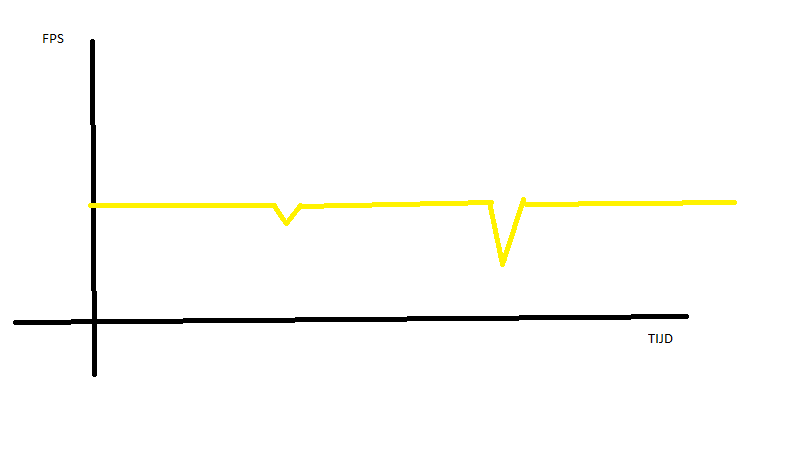
\includegraphics[width=\textwidth]{img/fpsgrafiek}\caption{FPS Van ARCore}\label{fig:fpsgr1}
\end{figure}
\section{Geheugen verbruik}
Sommatie nemen van de gemiddelde van elk tijdstip van elk experiment.
\begin{figure}
    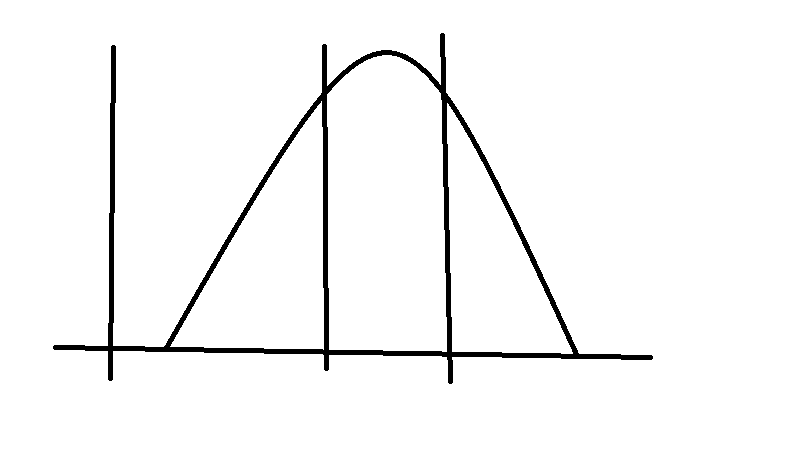
\includegraphics[width=\textwidth]{img/normaleverdeling}\caption{Geheugenverbruik Van ARCore}\label{fig:mem1}
\end{figure}
\section{Batterij verbruik}
Dit kan eigenlijk gewoon een tabel zijn waarin elk framework zijn batterij verbruik staat?
\section{Temperatuur}
Evolutie van temperatuur over tijd tonen?
\section{Afbeeldingsherkenning}
Elk framework zal ook een lijst krijgen van 10 afbeeldingen om te kijken hoe goed hij verschillende afbeeldingen kan herkennen. Hier zal er ook worden gekeken van hoever hij deze kan herkennen!
Een conclusie waarom bepaalde afbeeldingen niet worden herkent kan hier ook in komen
\begin{figure}
    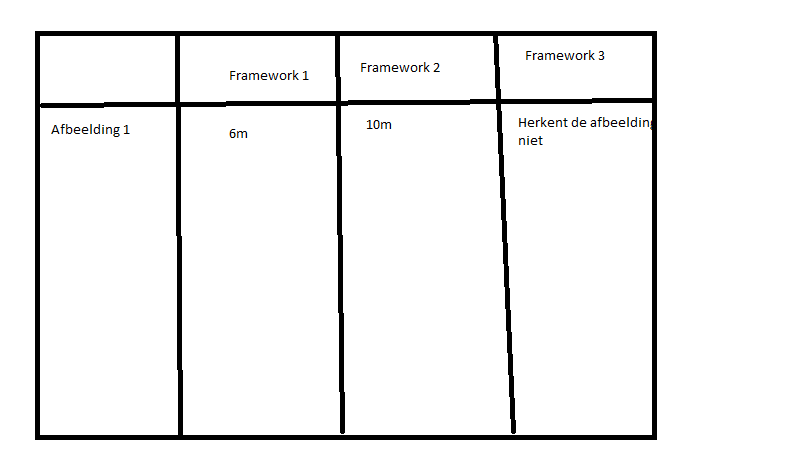
\includegraphics[width=\textwidth]{img/imgrex}\caption{Tabel aantal meter tot herkenning}\label{fig:imgrex}
\end{figure}
\section{Conclusie best scorend framework}
Hierin komt de conclusie over het best scorend framework en waarom deze de best scorende is. Hierin zal ook rekening worden gehouden met de score van het vorige hoofdstuk!